%---------------------------------------------------------------------------%
%->> Section 2.4: 大语言模型驱动的根因定位方法
%---------------------------------------------------------------------------%

\section{大语言模型驱动的根因定位方法}

传统方法在已知故障场景下取得了一定效果，但在动态环境中仍难以统一组织多源证据，也缺乏交互式诊断和历史经验的灵活复用。为缓解这些问题，研究者开始将大语言模型引入微服务故障根因定位任务，以期利用其语言理解和推理能力弥合不同模态之间的语义鸿沟。现有工作大致可分为四类：大语言模型离线分析、工具增强的单智能体、多智能体协同诊断，以及知识增强的多智能体协同诊断。

\subsection{大语言模型离线分析}

早期方法将大语言模型放在诊断流程末端。系统先完成告警聚合、诊断信息收集和上下文组织，再把整理后的材料交由大语言模型生成根因报告、故障摘要或处置建议。在这类方法中，大语言模型主要负责理解和组织已有证据，而不直接参与在线诊断过程。

Ahmed 等人\cite{ahmed2023recommending}较早系统评估了大语言模型在云故障根因与缓解建议生成中的可行性； GPT-4 上下文学习的自动根因分析方法\cite{zhang2024gpt4iclrca}表明，不依赖持续微调也能生成较高质量的根因建议。PACE-LM\cite{zhang2023pacelm}在推荐阶段加入置信度估计，以降低幻觉输出误导值班工程师的风险。X-lifecycle Learning\cite{goel2024xlifecycle}尝试将代码、配置和监控等信息统一纳入上下文；eARCO\cite{goel2025earco}进一步利用提示优化和相似案例增强改进推荐质量。这些工作说明，即使只在流程末端使用模型，大语言模型也能改善事件摘要、案例对齐和根因解释。

在系统实现层面，RCACopilot\cite{chen2024rcacopilot}将告警、运行时诊断信息与历史事件组织为统一输入，再由模型生成根因类别和解释性叙述；Xpert\cite{xpert-jiang2024}根据故障上下文推荐诊断查询，以减少人工编写运维 DSL 的工作量。Cloud Atlas\cite{xie2024cloud}利用大语言模型结合系统文档、遥测和部署信息自动构建因果图，并通过额外验证步骤提高可靠性。但这类方法处理的仍然是预先整理好的材料。一旦证据不足，模型既无法主动发起新的观测请求，也难以根据中途结果调整排查方向。后续工作因此转向让模型直接调用外部工具。

\subsection{工具增强的单智能体}

工具增强的单智能体方法将大语言模型引入诊断过程。与离线分析不同，这类方法不再只处理事先整理好的材料，而是让模型通过工具调用访问日志、指标、数据库或拓扑信息，并根据观察结果决定下一步动作。诊断过程因此由离线总结转向在线交互，模型从被动接收者转变为主动探索者。

在通用方法层面，ReAct\cite{yao2022react}为语言模型结合推理与行动提供了统一范式，ToolFormer 和 ToolLLM\cite{schick2024toolformer,qin2023toolllm}增强了模型调用外部工具和真实 API 的能力。在根因定位场景中，Roy 等人\cite{roy2024exploringllmrca}系统评估了配备检索与诊断服务接口的 ReAct 智能体，指出主动收集日志、指标和数据库信息能够缓解离线分析中的信息不足问题。RCAgent\cite{wang2024rcagent}在工业云环境中加入上下文管理、自一致动作序列和输出稳定化机制，使单智能体更接近真实可用。

后续工作主要围绕如何提高单智能体诊断稳定性来展开。K8sGPT\cite{k8sgpt2023}是较早的大语言模型辅助 Kubernetes 排障工具，它通过 analyzers 检查集群对象，并结合事件和资源状态生成诊断说明；SynergyRCA\cite{xiang2025synergyrca}用 StateGraph 和 MetaGraph 提供更结构化的 RCA 上下文。MicroRCA-Agent\cite{tang2025microrcaagent}将日志压缩、链路异常筛选和跨模态提示融合到统一流程中；GALA\cite{tian2025gala}则将结构化传播线索与语言推理结合起来。与离线分析相比，这类方法已经能够在诊断过程中持续观察、推理，并根据中途结果调整动作。

然而，这种方式的负担也逐渐集中到单个智能体内部。随着可调用工具和上下文范围不断扩大，日志检索、证据解释、工具选择、路径调整和结论生成等职责都压在同一个执行体上。动作链变长或上下文堆积时，系统稳定性就会明显下降\cite{roy2024exploringllmrca,wang2024rcagent,xiang2025synergyrca,tang2025microrcaagent}。这种单点负载过重的问题促使后续研究开始将不同职责拆分给多个角色。

\subsection{多智能体协同诊断}

多智能体协同诊断方法进一步把诊断过程拆分给多个角色。与工具增强的单智能体不同，这类方法不再由单个智能体承担日志检索、证据解释、路径选择和结论生成等全部职责，而是将告警理解、数据检索、依赖分析、根因判断和处置建议分配给不同角色，并利用角色之间的交叉验证降低单点推理失误带来的影响。

在通用研究中，MetaGPT\cite{hong2023metagpt}和 Multi-LLM Agent\cite{small-llm-agents}都表明，将复杂任务拆分为不同角色，通常比让单个模型承担全部职责更稳定。放到 RCA 场景中，mABC（Multi-Agent Blockchain-inspired Collaboration，多智能体区块链协同）\cite{zhang2024mabc}通过七类专用智能体组成协作流水线，并引入区块链式投票机制缓解单点幻觉；Nissist\cite{an2024nissist}围绕 TSG 理解、检索和计划生成构建多智能体故障处置辅助系统。相较于单智能体，这类方法的关键变化在于把错误风险分散到多个决策环节。

进一步的工作开始转向协作过程本身的控制。 Monte Carlo Tree Search 的多智能体故障定位系统\cite{ren2025mctsfaultlocalization}尝试用树搜索和知识奖励机制控制服务级探索顺序；RCLAgent\cite{zhang2025rclagent}借鉴人工 RCA 中递归展开和跨模态推理的特点，提出 multi-agent recursion-of-thought 框架。相应地，多智能体方法关注的已不只是角色分工，还包括协作方式和停止条件。

不过，多智能体并未从根本上消除诊断不稳定问题。角色数量增加后，消息传递、共享状态维护、协作顺序和停止条件都会成为新的系统负担。若机制设计不当，系统容易退化为冗长交互、重复取证，甚至出现不同角色相互冲突的判断，反而降低诊断效率。后续研究因此开始进一步引入 SOP、TSG、规则库和显式工作流，以减少开放式协作带来的不确定性。

\subsection{知识增强的多智能体协同诊断}

知识增强的多智能体协同诊断方法进一步把已有知识纳入诊断过程。与前一类方法相比，这类工作不再主要依赖角色之间的开放式协作，而是将排障指南、标准操作规程（Standard Operating Procedure，SOP）、故障排查指南（Troubleshooting Guide，TSG）和历史案例转化为执行约束，通过离线编译、在线检索或动作限制等方式缩小动作空间，从而提高诊断的稳定性和可预测性。

这类方法在知识使用方式上存在差异。LLexus\cite{lascasas2024llexus}将自然语言 TSG 转化为可执行计划，再让智能体按计划执行；Nissist\cite{an2024nissist}从 TSG 和历史缓解记录中抽取知识并构建知识库；Flow-of-Action\cite{pei2025flowofaction}通过 Thought-ActionSet-Action 范式，将 SOP 约束嵌入多智能体动作选择过程。共同点在于，已有经验不再只是参考材料，而被转化为角色需要遵守的执行约束。

\begin{figure}[tbp]
\centering
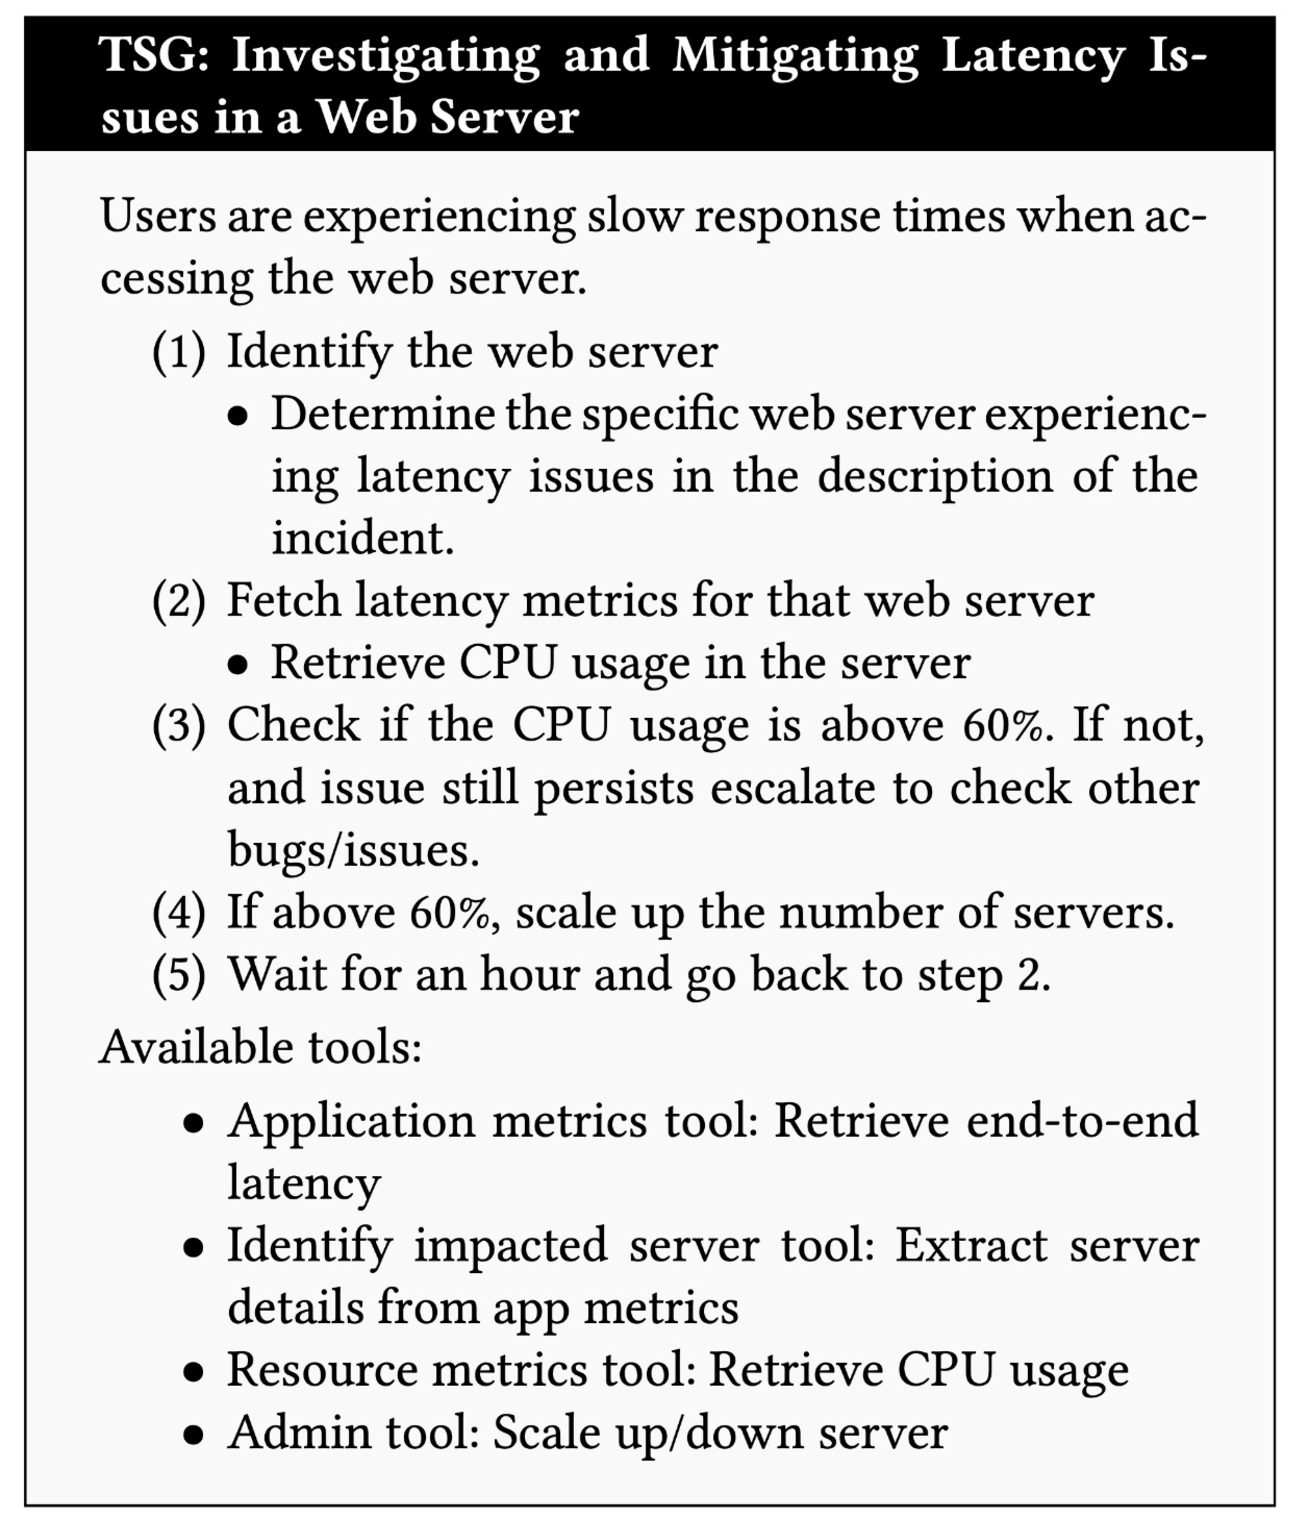
\includegraphics[width=0.54\textwidth]{Figures-Src/Chap2-RelatedWork/tsg/chart.pdf}
\bicaption{\enspace LLexus 中的 TSG 片段示例\cite{lascasas2024llexus}}{\enspace TSG Snippet from LLexus\cite{lascasas2024llexus}}
\label{fig:llexus_tsg_example}
\end{figure}

图\ref{fig:llexus_tsg_example}给出了 LLexus\cite{lascasas2024llexus} 中的一段 TSG。图中直接写出了问题描述、排查步骤和可调用工具，也说明这类方法对既有 TSG 的质量和覆盖范围依赖较强。

另一组工作更进一步，将知识直接编译为工作流。ARCAS\cite{demarne2024arcas}通过 DSL 化的 Auto-TSG 库组织并行诊断逻辑，再由 LLM 对多路输出进行优先级判断；StepFly\cite{mao2025agentictsgautomation}将 TSG 质量改进、执行 DAG 抽取和在线 scheduler-executor 执行整合在一起。FastReject\cite{fastreject2025}则体现出“在线诊断 + 离线规则演进”的思路。发展到这一步，知识已不再只是辅助材料，而成为诊断流程的一部分。

但这类方法仍未彻底解决问题。知识增强确实提升了稳定性，但许多系统仍依赖人工整理或离线整理好的 SOP、TSG 和规则库，因此知识获取与更新成本较高\cite{an2024nissist,lascasas2024llexus,mao2025agentictsgautomation}。近期针对 RCA 智能体的过程级失败分析也表明，即便加入知识约束，数据解释错误、探索不完整和角色通信失效等问题仍然存在\cite{kim2026agentfailurerca}。总体上，现有工作大多仍停留在调用既有 SOP、TSG 和规则库，而缺乏从真实诊断过程中自动提取和演化知识的能力。稳定的故障表征、从真实诊断过程自动生成 SOP 的方法，以及把 SOP 在线执行、必要探索和后续更新串联起来的机制，仍然是有待解决的三个基础问题。第三章正是围绕这三点展开。
